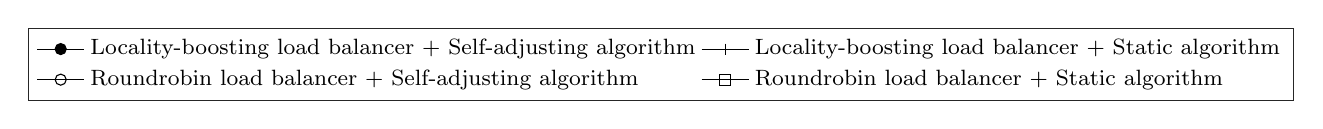
\begin{tikzpicture} 
  \begin{axis}[%
    height=45pt,
    hide axis,
    xmin=10,
    xmax=50,
    ymin=0,
    ymax=0.4,
    legend style={
      draw=white!15!black,
      legend cell align=left,
      legend columns=2,
      font=\footnotesize}
    ]
    \addlegendimage{black,mark=*}
    \addlegendentry{Locality-boosting load balancer + Self-adjusting algorithm}
    \addlegendimage{black,mark=+}
    \addlegendentry{Locality-boosting load balancer + Static algorithm}
    \addlegendimage{black,mark=o}
    \addlegendentry{Roundrobin load balancer + Self-adjusting algorithm}
    \addlegendimage{black,mark=square}
    \addlegendentry{Roundrobin load balancer + Static algorithm}
  \end{axis}
\end{tikzpicture}

%%% Local Variables:
%%% mode: latex
%%% TeX-master: "../distributed_mrf"
%%% End:
